\documentclass{my_cv}
\usepackage[left=3cm,right=3cm,top=1cm,bottom=1cm]{geometry}
\usepackage{fontawesome}
\usepackage{graphicx}
\usepackage{url}
\usepackage{fontspec}
\usepackage{color,xcolor}

\setmainfont{Georgia}
\begin{document}
	\thispagestyle{empty}
	\noindent
	\begin{minipage}[t]{.5\linewidth}
		\raggedright 
		\vspace{-2cm}
		{\bfseries \Huge Zhihao Yao}\\
		\small\itshape
		\faHome \hspace{1mm}  Elsterstraße 12, 04109, Leipzig\\
		\faMobilePhone\hspace{1mm} +49-151-12734936\\
		\faEnvelopeO \hspace{1mm} zyao2015inf@gmail.com\\
		\faSkype \hspace{1mm} live:yzh2015summer
	\end{minipage}
	\begin{minipage}[t]{.5\linewidth}
		\raggedleft 
		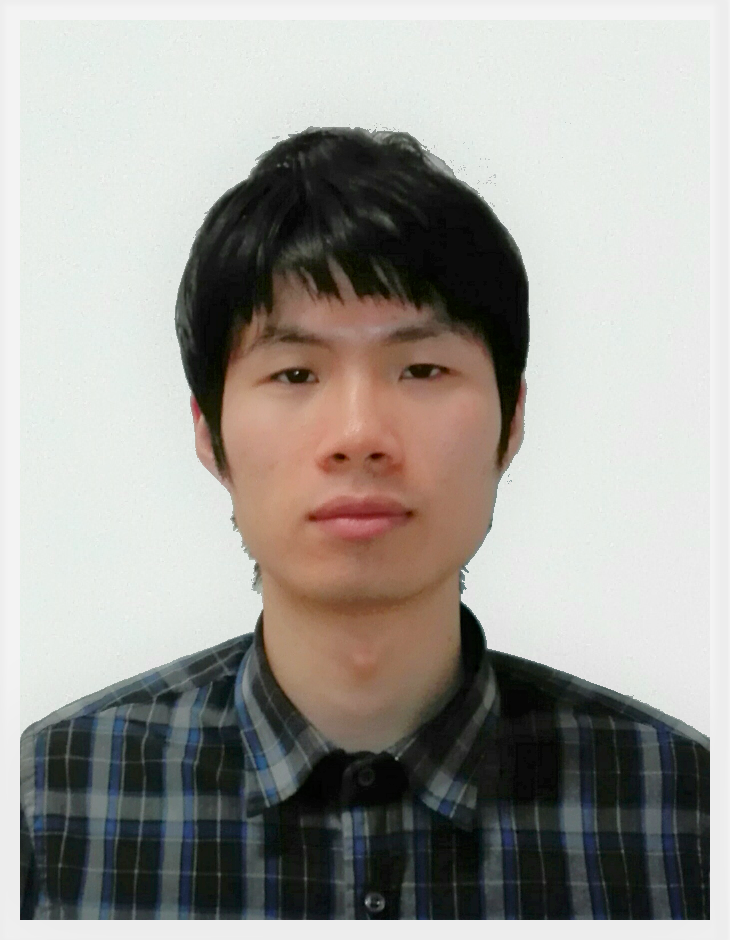
\includegraphics[width=.3\linewidth]{bewerbung.png}
	\end{minipage}
	\section{\faMale\ Personal Description}
	My full name is Zhihao Yao, I was born on 29.07.1993 in Maanshan, a city situated in the south-east of China. After my successful (also fulfilling) studies major in Master of Computational Logic, TU Dresden, I am confident that I have qualifications for both practical and theoretical tasks related to Semantic Web.
	\section{\faGraduationCap\ Education}
	\datedsubsection{Technische Universität Dresden}{2015.10--2019.2}
	Master of Science, Computational Logic, Graduation Grade: \textbf{1.7}.
	\datedsubsection{Anhui University of Technology in China}{2011.9--2015.7}
	Bachelor of Engineering, Computer Science and Technology, Graduation Grade: \textbf{2.0} (According to the German Grading System). 
	\section{\faBriefcase\ Experience}
	\datedsubsection{Exchange Student}{2016.3--2016.7}
	Half-year study at the {\itshape Free University of Bozen-Bolzano, Italy}. Worked in a group of three people as required by mini projects. Scheduled the job assignment as well as contributing to coding and presentation. 
	\datedsubsection{Teaching Assistant}{2018.1--2018.2}
	Tutor of the tutorial for the course {\itshape``Science of Computational Logic"}. Taught tutorials to over 20 students and assisted in grading exam papers. 
	\section{\faFolderOpen\ Projects}
	\datedsubsection{Computing Minimal DL-model Using First-Order Model Finders}{2017.4--2017.11}
	Developed a Java program to translate OWL Ontologies into files in TPTP (Thousands of Problems for Theorem Provers) format. Presented an evaluation result for different model finders.\\
	\faGithub\  \url{https://github.com/ZhYao2015/2017summer/tree/master/owl2tptp}
	\datedsubsection{An ASP-Based SPARQL Query Engine}{2018.4--2018.12}
	Developed a Java implementation of a method based on an independent work, which translates SPARQL Queries into Answer Set Programs. Proved the correctness of the modified translation under certain semantics proposed by my supervisor and presented a preliminary evaluation as well.\\
	\faGithub\ \url{https://github.com/ZhYao2015/sparql-experimental}
	\section{\faKey\ Skills}
	\begin{itemize}
		\item Artificial Intelligence: Knowledge Graphs ( OWL, SPARQL, Prot\'{e}g\'{e} ), Machine Learning
		\item Others: Java, HTML/CSS/JS, \LaTeX
	\end{itemize}
	\section{\faGlobe\ Languages}
	\vspace{-5mm}
	\begin{table}[h]
		\begin{tabular}{lll}
			{\bfseries \Large English}&{\bfseries \Large Chinese}&{\bfseries \Large German}\\
			Proficient & Native speaker & Elementary\\
		\end{tabular}
	\end{table}
\end{document}